\documentclass[conference,a4paper]{IEEEtran}
\IEEEoverridecommandlockouts

\usepackage[T1]{fontenc}
\usepackage{cite}
\usepackage{amsmath,amssymb}
\usepackage{booktabs}
\usepackage{graphicx}
\usepackage[dvipsnames]{xcolor}
\usepackage{tikz}
\usetikzlibrary{positioning,arrows.meta,fit,backgrounds,calc}
\usepackage{pgfplots}
\pgfplotsset{compat=1.18}
\usepackage{url}
\usepackage[hidelinks]{hyperref}

% Okabe-Ito colours (colour-blind safe)
\definecolor{cblue}{HTML}{0072B2}
\definecolor{corange}{HTML}{E69F00}
\definecolor{cgreen}{HTML}{009E73}
\definecolor{cgrey}{HTML}{777777}
\definecolor{boxfill}{HTML}{F2F5F9}

\newcommand{\logit}{\operatorname{logit}}
\newcommand{\BSS}{\mathrm{BSS}}

\begin{document}

\title{Forecasting Big Fire Days in Iberia:\\ Satellite Fire History, Fire Weather and an Honest\\ Evaluation with Real Forecast Errors}

\author{\IEEEauthorblockN{Birk Wipke, Leni Ohle, Yannis Brassat, Jonathan Richter, Christoph Gahabka}
\IEEEauthorblockA{NASA Space Apps Challenge 2026, ``MODIS and VIIRS Hot Spots''}}

\maketitle

\begin{abstract}
Wildfire activity on the Iberian Peninsula is concentrated on few days: 2.9\,\% of all region-days carry 91\,\% of the
fire radiative power (FRP) observed by satellite. We forecast, for 23 NUTS-2 regions, the probability of such a
\emph{big fire day} (harmonised VIIRS FRP $\geq 100$\,MW) 1 to 10 days ahead, and give a three-class outlook for
weeks 2--4. Each lead time has its own ridge-penalised logistic regression. Its inputs are a smoothed seasonal
climatology, the fire history up to the issue date and 22 fire-weather features derived from ERA5 (Canadian Fire
Weather Index system, Fosberg index, anomalies). In operation the model only sees \emph{forecast} weather, so we train
and test it on weather perturbed with real ECMWF IFS forecast errors. On validation, a model trained on perfect weather
fell below the model without weather (Brier skill 0.024 vs.\ 0.048), while error-aware training reached 0.093. On the
test years 2022--2026 the honest Brier skill score against climatology is 0.25 at day~1, 0.11 at day~5 and 0.05 at
day~10 (AUC 0.94--0.89), with an expected calibration error of at most 0.009. A shipping rule falls back to
climatology wherever the skill is not significant.
\end{abstract}

\begin{IEEEkeywords}
wildfire forecasting, VIIRS, fire radiative power, Fire Weather Index, logistic regression, forecast verification
\end{IEEEkeywords}

% ===========================================================================
\section{Introduction}

Satellite active fire products record where and when vegetation burns \cite{schroeder2014,giglio2016}. In the La-Brasa
web application we harmonise the NASA FIRMS hotspots of MODIS and VIIRS \cite{firms} into one daily record per NUTS-2
region and show it on a map and a calendar. This paper describes the forecast module built on top of that record. It
answers one question per region and day: \emph{how likely is a day with strong fire activity in the next ten days?}

Two facts shape the design. First, fire activity is persistent: a region that burns today is three times more likely to
burn tomorrow than the season suggests. Second, the weather decides the days after that, but in operation only a
\emph{forecast} of it is available. Most published skill numbers for weather-driven models are measured with observed
or reanalysed weather on the target day, which overstates operational skill.

\textbf{Contributions.} (i) Lead-specific, calibrated logistic models that combine fire history, a shrunk seasonal
climatology and fire-weather features, implemented without external ML libraries. (ii) An honest evaluation in which
the forecast weather of every lead carries real IFS forecast errors, and the finding that error-aware training is
necessary for weather features to help at all. (iii) An operational chain with a statistical shipping rule, risk
classes and an uncertainty band from a 51-member ensemble.

% ===========================================================================
\section{Related Work}

Fire danger in Europe is usually expressed by the Canadian Fire Weather Index (FWI) system
\cite{vanwagner1985,vanwagner1987}. In Iberia, FWI depends on the reanalysis used \cite{bedia2012}, and extreme
fire-weather days track burnt area \cite{calheiros2020}. Driven by numerical weather prediction, FWI keeps useful skill
for up to about ten days \cite{digiuseppe2016,digiuseppe2020}. These systems forecast fire \emph{danger}, not observed
activity. Data-driven work predicts next-day danger or spread with deep learning
\cite{kondylatos2022,kondylatos2023,huot2022}, mostly with observed predictors. Statistical post-processing in
meteorology distinguishes ``perfect prog'' models, which are trained on observations \cite{klein1959}, from Model Output
Statistics, which are trained on forecasts \cite{glahn1972}. Our error-aware training sits between the two.

% ===========================================================================
\begin{figure*}[t]
\centering
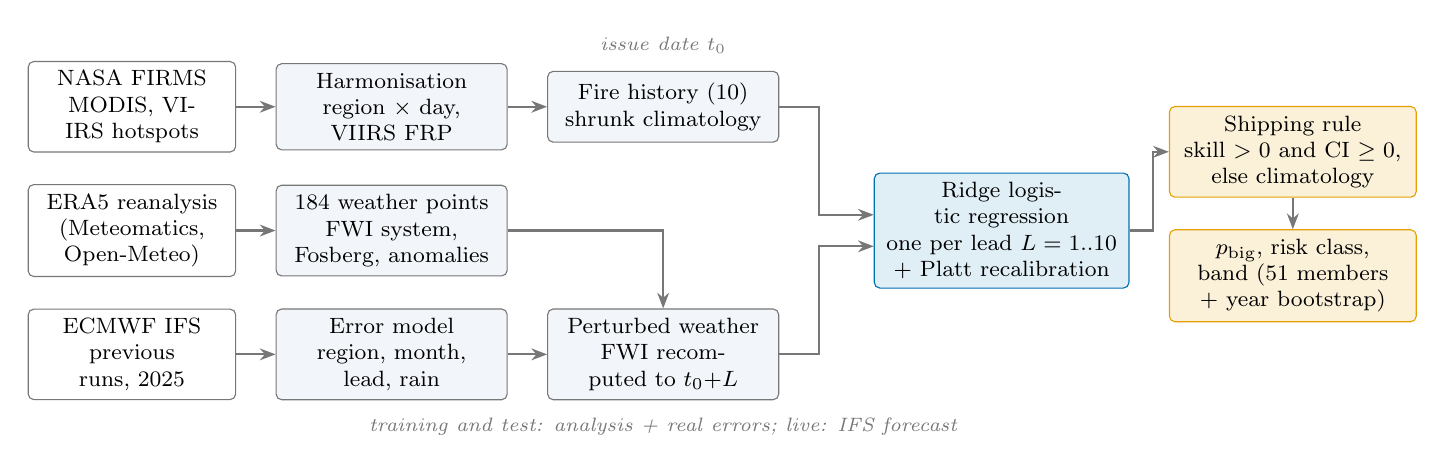
\begin{tikzpicture}[
  font=\footnotesize, node distance=4mm and 5mm,
  box/.style={draw=cgrey, fill=boxfill, rounded corners=2pt, align=center, minimum height=9mm, text width=27mm},
  src/.style={box, fill=white, text width=24mm},
  mdl/.style={box, fill=cblue!12, draw=cblue, text width=30mm},
  outbox/.style={box, fill=corange!15, draw=corange, text width=29mm},
  arr/.style={-{Stealth[length=2mm]}, thick, cgrey},
  lbl/.style={font=\scriptsize\itshape, text=cgrey}]
  % inputs
  \node[src] (firms) {NASA FIRMS\\MODIS, VIIRS hotspots};
  \node[src, below=of firms] (era5) {ERA5 reanalysis\\(Meteomatics, Open-Meteo)};
  \node[src, below=of era5] (ifs) {ECMWF IFS\\previous runs, 2025};
  % processing
  \node[box, right=of firms] (harm) {Harmonisation\\region $\times$ day, VIIRS FRP};
  \node[box, right=of era5] (wx) {184 weather points\\FWI system, Fosberg, anomalies};
  \node[box, right=of ifs] (err) {Error model\\region, month, lead, rain};
  \node[box, right=of harm] (hist) {Fire history (10)\\shrunk climatology};
  \node[box, right=of err] (pert) {Perturbed weather\\FWI recomputed to $t_0{+}L$};
  % model and outputs
  \node[mdl, right=12mm of $(hist.east)!0.5!(pert.east)$] (model) {Ridge logistic regression\\one per lead $L=1..10$\\+ Platt recalibration};
  \node[outbox, right=of model, yshift=10mm] (rule) {Shipping rule\\skill $>0$ and CI $\geq 0$,\\else climatology};
  \node[outbox, below=of rule] (prod) {$p_\text{big}$, risk class,\\band (51 members\\+ year bootstrap)};
  % arrows
  \draw[arr] (firms) -- (harm);
  \draw[arr] (harm) -- (hist);
  \draw[arr] (era5) -- (wx);
  \draw[arr] (ifs) -- (err);
  \draw[arr] (err) -- (pert);
  \draw[arr] (wx.east) -| (pert.north);
  \draw[arr] (hist.east) -- ++(5mm,0) |- ([yshift=2mm]model.west);
  \draw[arr] (pert.east) -- ++(5mm,0) |- ([yshift=-2mm]model.west);
  \draw[arr] (model.east) -- ++(3mm,0) |- (rule.west);
  \draw[arr] (rule) -- (prod);
  % live path
  \node[lbl, below=1mm of pert] {training and test: analysis + real errors; live: IFS forecast};
  \node[lbl, above=1mm of hist] {issue date $t_0$};
\end{tikzpicture}
\caption{Architecture of the forecast module. Fire history and climatology come from the harmonised hotspot record;
weather features are computed per weather point and averaged per region. For training and testing, the weather between
issue date $t_0$ and target day $t_0+L$ is perturbed with real forecast errors; live, the IFS forecast is used instead.}
\label{fig:arch}
\end{figure*}

% ===========================================================================
\section{Data}

\subsection{Fire record and targets}
The input is the harmonised daily table of the La-Brasa pipeline: one row per NUTS-2 region and day, with detection
counts and FRP per satellite, and the harmonised FRP, i.e.\ the mean over the active VIIRS satellites (SNPP, NOAA-20,
NOAA-21). The forecast uses only days measured by VIIRS (20.01.2012 to 13.11.2026) in 23 regions of mainland Spain,
Portugal and south-western France (Table~\ref{tab:data}).

\emph{Big fire day:} harmonised FRP $\geq 100$\,MW in a region on one day. It is rare (2.87\,\%) but holds 91\,\% of the
FRP. \emph{Fire day:} any detection by SNPP. We do not use ``any detection by any VIIRS satellite'', because this share
grows with the number of satellites in orbit (0.33 in 2017, 0.42 in 2019 after NOAA-20 joined, while SNPP alone stayed
at 0.32). That is a measurement effect, not a trend.

\begin{table}[t]
\centering
\caption{Forecast data set (VIIRS-measured region-days).}
\label{tab:data}
\footnotesize
\begin{tabular}{@{}lr@{}}
\toprule
Regions (NUTS-2) & 23 \\
Region-days, 20.01.2012--13.11.2026 & 124\,108 \\
\quad training 2012--2021 / test 2022--2026 & 83\,490 / 40\,618 \\
Big fire days (train / test) & 2\,385 / 1\,181 \\
Base rate big fire day / fire day (SNPP) & 2.87\,\% / 27.8\,\% \\
Share of FRP on big fire days & 90.6\,\% \\
Big fire days June--October & 64.5\,\% \\
Episodes of big fire days: mean length / single day & 1.66\,d / 71\,\% \\
Weather points (8 per region) & 184 \\
\bottomrule
\end{tabular}
\end{table}

\subsection{Persistence and seasonality}
Big fire days cluster in time. Fig.~\ref{fig:persist} compares the probability of a big fire day $L$ days after
another one with the climatological probability on the same days. The lift is 3.1 at one day, 1.7 at five days and
1.2 at ten days. Running fires therefore carry the first days of the forecast. The season is strong as well: 64.5\,\%
of big fire days fall in June to October. Six northern regions, however, peak in February or March (agricultural and
pasture burning), so the seasonal curve must be regional.

\begin{figure}[t]
\centering
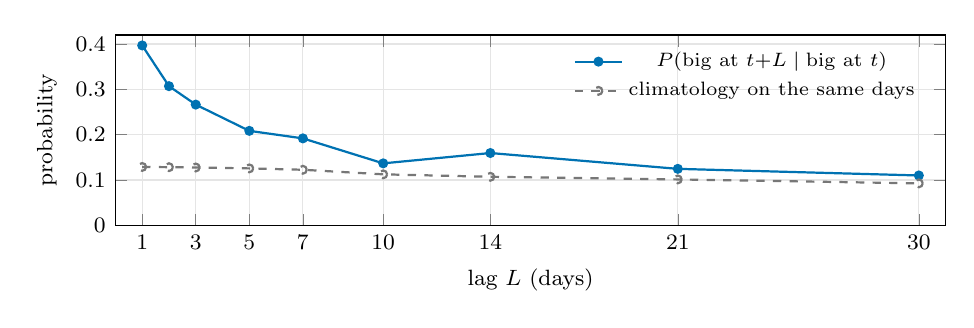
\begin{tikzpicture}
\begin{axis}[
  width=\columnwidth, height=40mm, font=\footnotesize,
  xlabel={lag $L$ (days)}, ylabel={probability},
  xmin=0, xmax=31, ymin=0, ymax=0.42, xtick={1,3,5,7,10,14,21,30},
  legend style={draw=none, fill=none, at={(0.98,0.97)}, anchor=north east, font=\scriptsize},
  grid=major, grid style={gray!20}]
\addplot[thick, cblue, mark=*, mark size=1.4pt] coordinates
  {(1,0.3969) (2,0.3071) (3,0.2664) (5,0.2085) (7,0.1919) (10,0.1368) (14,0.1596) (21,0.1247) (30,0.1101)};
\addlegendentry{$P(\text{big at } t{+}L \mid \text{big at } t)$}
\addplot[thick, cgrey, dashed, mark=o, mark size=1.4pt] coordinates
  {(1,0.1289) (2,0.1284) (3,0.1277) (5,0.1257) (7,0.1227) (10,0.1126) (14,0.1072) (21,0.1014) (30,0.0927)};
\addlegendentry{climatology on the same days}
\end{axis}
\end{tikzpicture}
\caption{Persistence of big fire days (training years). After a big fire day the next one is 3.1 times as likely as
the season implies; the excess fades within about ten days.}
\label{fig:persist}
\end{figure}

\subsection{Weather}
Regions are large (Andaluc\'{i}a covers about 87\,000\,km$^2$), and a regional mean would dilute the weather where fires
burn. We therefore use per region the eight $0.25^\circ$ cells with the most VIIRS detections in 2012--2021, weighted by
their share of detections. Daily values at 12~UTC come from ERA5 \cite{hersbach2020} for the history and from the
ECMWF IFS for the forecast. An automatically mixed source from the first provider had implausible precipitation
(42\,mm instead of about 1\,400\,mm in Galicia in 2023), so the history was reloaded from ERA5. In the fire season the
FWI anomaly separates big fire days best among single weather features (AUC 0.76 within region and month).

% ===========================================================================
\section{Method}

\subsection{Problem and climatology}
For region $r$, issue date $t_0$ and lead $L \in \{1,\dots,10\}$ we estimate
$p_{r,t_0,L} = \Pr(Y_{r,t_0+L} = 1 \mid \text{data up to } t_0)$. We use the direct approach: one model per target and
lead, trained on pairs (features at $t_0$, target at $t_0+L$), so errors do not accumulate over leads.

The reference forecast and strongest single input is a seasonal climatology per region and day of year $d$. A hard
$\pm 7$-day window left 37\,\% of region-days at the minimum value, so we shrink a narrow kernel rate towards a broad
one:
\begin{equation}
c_r(d) = \frac{S_r(d) + m\,P_r(d)}{N_r(d) + m},
\end{equation}
where $S_r$ and $N_r$ are event and observation counts smoothed with a circular Gaussian kernel ($\sigma = 10$ days),
$P_r$ is the same rate with $\sigma = 30$ days, and $m = 20$ pseudo-days for big fire days. It enters the model as
$\logit c_r(d)$, so the model can reproduce the climatology exactly.

\subsection{Features}
\emph{Fire history at $t_0$} (10 features): $\log(1{+}\text{FRP})$ on the last day and as means over 3, 7 and 30 days;
fire-day share over 7 and 30 days; big-fire-day share over 30 days; log days since the last big fire day; FRP of the
three nearest regions. All windows end at $t_0$.

\emph{Weather of the target day} (22 features), computed from base variables only (temperature, humidity, wind, gusts,
precipitation, dew point): the six FWI codes FFMC, DMC, DC, ISI, BUI and FWI \cite{vanwagner1985}, our own Fosberg
index \cite{fosberg1978,goodrick2002}, maximum temperature, humidity, vapour pressure deficit, gusts, rain, days since
rain, 30-day rain, 90-day rain anomaly, anomalies of FWI, DC, maximum temperature and VPD, and three nonlinear terms
($\log\text{FWI} \times \logit c$, $\text{DC} \times \logit c$, $(\log\text{FWI})^2$). The interaction lets a high FWI
act differently in winter and summer. Our FWI implementation matches the published test table of
\cite{vanwagner1985} to within 0.005. Inputs are standardised; regions enter as penalised one-hot effects.

\subsection{Model}
With design vector $\mathbf x_i$ and $p_i = \sigma(\mathbf x_i^\top \mathbf w)$ we maximise the ridge-penalised
log-likelihood \cite{lecessie1992}
\begin{equation}
\ell_\lambda(\mathbf w) = \sum_i \big[y_i \eta_i - \log(1 + e^{\eta_i})\big] - \tfrac12 \mathbf w^\top \Lambda \mathbf w,
\quad \eta_i = \mathbf x_i^\top \mathbf w,
\end{equation}
by Newton--Raphson (IRLS) in plain NumPy. $\Lambda$ is diagonal: 0 for the intercept, 100 for continuous inputs and 20
for region effects, chosen on validation. The output is recalibrated with Platt scaling
\cite{platt1999,niculescu2005}, $\tilde p = \sigma(a + b \logit p)$, fitted on the last two training years.

\subsection{Error-aware training}
For a forecast from $t_0$ to $t_0+L$, each forecast day $k = 1,\dots,L$ receives a real error vector, drawn jointly for
all variables so that their dependence is kept. The errors are IFS minus ERA5 for 2025 from the Open-Meteo Previous
Runs archive \cite{openmeteo}, matched by region, month $\pm 1$, lead and whether ERA5 had rain ($\geq 1$\,mm). Values
are clipped to physical bounds. The FWI codes are then propagated from the analysed state at $t_0$ through the perturbed
days, so the drought codes of the target day carry the accumulated error. Table~\ref{tab:errors} shows how the errors
grow with lead. Leads 8--9 (beyond the archive) extrapolate the growth of days 4--7. A per-region, per-month and
per-lead bias correction is applied in the same way as in live operation. Training with input noise acts like a
regulariser \cite{bishop1995}. Here the noise also has the size the model will meet in practice.

\begin{table}[t]
\centering
\caption{Standard deviation of IFS $-$ ERA5 errors (2025, 23 regions).}
\label{tab:errors}
\footnotesize
\begin{tabular}{@{}lcccc@{}}
\toprule
Lead (d) & Temp.\ ($^\circ$C) & Hum.\ (\%) & Wind (km/h) & Rain (mm) \\
\midrule
0 & 1.49 & 8.4 & 4.4 & 3.4 \\
3 & 1.81 & 9.9 & 5.1 & 4.0 \\
5 & 2.36 & 12.5 & 6.1 & 5.2 \\
7 & 2.99 & 14.5 & 7.2 & 5.9 \\
\bottomrule
\end{tabular}
\end{table}

\subsection{Shipping rule, risk classes and uncertainty}
A model is shipped for a lead only if its test skill against climatology is positive \emph{and} the lower bound of the
90\,\% year-bootstrap interval is $\geq 0$; otherwise the climatology is shipped and labelled as such. Regions with at
least 30 test events get their own decision. Risk classes follow the ratio $p / c$ (thresholds 0.67, 1.5, 3, 6), with
$p \geq 0.25$ at least ``high'', $p \geq 0.5$ ``very high'' and $p < 0.02$ at most ``normal''. The band
$[p_\text{lo}, p_\text{hi}]$ is the wider of the 5--95\,\% range over the 51 members of the ECMWF ensemble and the range
of 20 refits on resampled years. Weeks 2--4 use a penalised multinomial regression on terciles of weekly activity
(below, normal, above usual).

% ===========================================================================
\section{Experimental Setup}

Training covers 20.01.2012--31.12.2021 and the test 01.01.2022--31.07.2026 (last archive day). All choices (penalties,
feature set, error-aware training, bias correction, climatology) were made on a validation split (fit 2012--2019,
validate 2020--2021) and never on the test years. Test rows receive three independent error draws. Skill is the Brier
skill score \cite{brier1950} against the climatology,
$\BSS = 1 - \mathrm{BS}_\text{model} / \mathrm{BS}_\text{clim}$, and the ranked probability skill score for the weekly
outlook \cite{epstein1969,weigel2007}. Because the events are rare we report PR-AUC next to ROC-AUC \cite{saito2015},
and we report the expected calibration error (ECE) \cite{guo2017} and the calibration slope. The 90\,\% intervals come
from 1\,000 bootstrap replicates over whole years, a block bootstrap for dependent data \cite{kunsch1989,roberts2017}.
Acceptance thresholds (e.g.\ day-1 skill $\geq 0.10$, AUC $\geq 0.87$, ECE $\leq 0.015$) were fixed before the first
measurement.

% ===========================================================================
\section{Results}

\begin{table*}[t]
\centering
\caption{Big fire day, test 2022--2026. Skill against climatology without weather and with weather carrying real
forecast errors (``honest''); upper bound with perfect weather. Hit / false-alarm ratio for a warning on the top 10\,\%
of predictions.}
\label{tab:results}
\footnotesize
\setlength{\tabcolsep}{4.5pt}
\begin{tabular}{@{}c c c c c c c c c@{}}
\toprule
Lead & BSS no weather & \textbf{BSS honest} (90\,\% CI) & BSS perfect wx & AUC & PR-AUC & ECE & Slope & Hit / FAR \\
\midrule
1  & 0.213 & \textbf{0.250} (0.221--0.273) & 0.255 & 0.943 & 0.51 & 0.006 & 1.08 & 0.79 / 0.77 \\
3  & 0.078 & \textbf{0.147} (0.121--0.176) & 0.154 & 0.925 & 0.40 & 0.008 & 1.13 & 0.73 / 0.79 \\
5  & 0.037 & \textbf{0.109} (0.086--0.135) & 0.123 & 0.916 & 0.34 & 0.008 & 1.06 & 0.69 / 0.81 \\
7  & 0.020 & \textbf{0.077} (0.060--0.097) & 0.092 & 0.905 & 0.29 & 0.008 & 1.07 & 0.66 / 0.82 \\
10 & 0.005 & \textbf{0.053} (0.034--0.076) & 0.068 & 0.893 & 0.25 & 0.008 & 1.03 & 0.63 / 0.83 \\
\midrule
\multicolumn{9}{@{}p{0.97\textwidth}@{}}{Climatology alone: AUC 0.851. Fire day (SNPP), honest BSS: 0.178 / 0.122 / 0.073 at leads 1 / 5 / 10 (without weather 0.124 / 0.038 / 0.024), ECE $\leq 0.012$.}\\
\bottomrule
\end{tabular}
\end{table*}

\subsection{Daily forecasts}
Table~\ref{tab:results} and Fig.~\ref{fig:skill} summarise the test results. Without weather, skill comes almost
entirely from persistence and fades from 0.21 at day~1 to 0.005 at day~10. With honest forecast weather the model
beats the no-weather model at every lead: about three times the skill at day~5 and ten times at day~10. The gap to the
perfect-weather upper bound grows with lead (0.005 at day~1, 0.015 at day~10), as expected from the growing forecast
errors. All leads are well calibrated (ECE $\leq 0.009$, slope 1.03--1.13). The day-1 model beats climatology in every
one of the 15 years under leave-one-year-out (skill 0.12--0.31).

\begin{figure}[t]
\centering
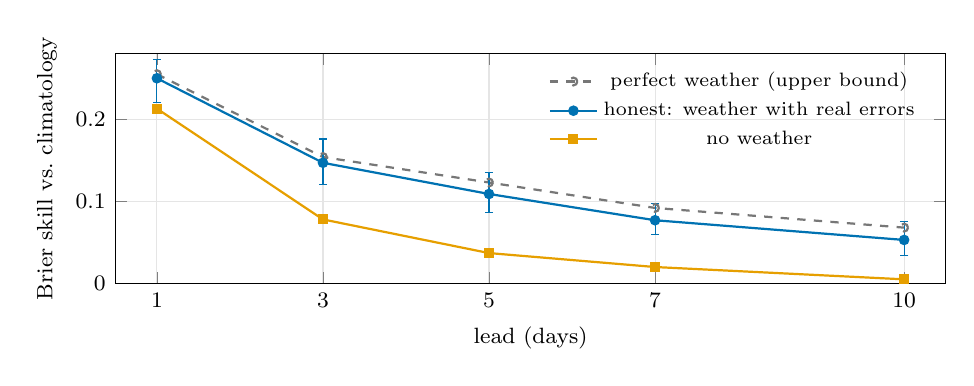
\begin{tikzpicture}
\begin{axis}[
  width=\columnwidth, height=45mm, font=\footnotesize,
  xlabel={lead (days)}, ylabel={Brier skill vs.\ climatology},
  xmin=0.5, xmax=10.5, ymin=0, ymax=0.28, xtick={1,3,5,7,10},
  legend style={draw=none, fill=none, at={(0.98,0.97)}, anchor=north east, font=\scriptsize},
  grid=major, grid style={gray!20}]
\addplot[thick, cgrey, dashed, mark=o, mark size=1.4pt] coordinates {(1,0.255) (3,0.154) (5,0.123) (7,0.092) (10,0.068)};
\addlegendentry{perfect weather (upper bound)}
\addplot[thick, cblue, mark=*, mark size=1.5pt, error bars/.cd, y dir=both, y explicit] coordinates {
  (1,0.250) += (0,0.023) -= (0,0.029)
  (3,0.147) += (0,0.029) -= (0,0.026)
  (5,0.109) += (0,0.026) -= (0,0.023)
  (7,0.077) += (0,0.020) -= (0,0.017)
  (10,0.053) += (0,0.023) -= (0,0.019)};
\addlegendentry{honest: weather with real errors}
\addplot[thick, corange, mark=square*, mark size=1.4pt] coordinates {(1,0.213) (3,0.078) (5,0.037) (7,0.020) (10,0.005)};
\addlegendentry{no weather}
\end{axis}
\end{tikzpicture}
\caption{Skill over lead time on the test years. Error bars: 90\,\% intervals from a bootstrap over years.}
\label{fig:skill}
\end{figure}

\subsection{Why error-aware training matters}
Table~\ref{tab:ablation} shows the central finding. A model trained on perfect weather relies heavily on the
target-day weather. Faced with forecast errors it is confidently wrong and ends up \emph{below} the model without weather.
Trained on weather with realistic errors, each lead-specific model learns how much the weather at that lead can be
trusted. This is the classic argument for Model Output Statistics over perfect-prog models \cite{glahn1972,klein1959}.

\begin{table}[t]
\centering
\caption{Validation 2020--2021, big fire day, mean skill over leads 1, 3, 5, 7, 10, scored with forecast errors.}
\label{tab:ablation}
\footnotesize
\begin{tabular}{@{}lc@{}}
\toprule
Variant & Mean BSS \\
\midrule
No weather & 0.048 \\
Weather, trained on perfect weather & 0.024 \\
Weather, trained with real forecast errors & 0.093 \\
\quad + IFS bias correction (selected) & \textbf{0.096} \\
\midrule
Upper bound: trained and scored on perfect weather & 0.115 \\
\bottomrule
\end{tabular}
\end{table}

\subsection{Risk classes, regions and weekly outlook}
The risk classes separate the outcomes cleanly (Table~\ref{tab:risk}). At day~1, ``very high'' days end as a big
fire day in 54\,\% of cases and ``low'' days in 0.9\,\%. Per region, the rule ships climatology for Madrid (ES30) at all
leads and for ES61 and ES52 from day 4 or 5 on. For ES51 and PT18 it alternates between neighbouring leads, because the
lower bound lies within $\pm 0.004$ of zero. The weekly outlook gains little: RPSS 0.020 (0.009--0.033) in week~2,
0.009 in week~3 and 0.002 in week~4, where climatology is shipped. Weather does not improve it.

\begin{table}[t]
\centering
\caption{Risk classes on the test years: share of region-days in the class / frequency of a big fire day.}
\label{tab:risk}
\footnotesize
\begin{tabular}{@{}lccc@{}}
\toprule
Class & Lead 1 & Lead 5 & Lead 10 \\
\midrule
low       & 57\,\% / 0.9\,\% & 57\,\% / 1.1\,\% & 55\,\% / 1.3\,\% \\
normal    & 36\,\% / 1.6\,\% & 36\,\% / 2.7\,\% & 40\,\% / 3.2\,\% \\
elevated  & 3.0\,\% / 11\,\% & 3.9\,\% / 11\,\% & 3.2\,\% / 11\,\% \\
high      & 2.2\,\% / 25\,\% & 2.3\,\% / 25\,\% & 1.5\,\% / 27\,\% \\
very high & 1.7\,\% / 54\,\% & 0.6\,\% / 37\,\% & 0.1\,\% / 44\,\% \\
\bottomrule
\end{tabular}
\end{table}

\subsection{Operation}
Training (feature selection, evaluation, production models and bootstrap) takes 6.4\,min on one core. The daily
prediction including the 51-member ensemble takes 7\,s with 1.1\,GB of memory. A daily job fetches the weather, runs
the prediction and keeps the last valid output if a contract check fails. Two runs give bit-identical outputs.

% ===========================================================================
\section{Discussion and Limitations}

The forecast covers \emph{detected fire activity} per region, not single fires or burnt area. Most Iberian fires are
started by people, so the model says how favourable conditions are, not whether a fire will be lit. The error model is
built from one year (2025) and one point per region, while the model averages up to eight points; the honest skill is
therefore rather conservative. Errors on consecutive days are drawn independently, whereas real forecast errors are
correlated, which may make the drought codes slightly optimistic. Weekly activity drifts with the number of VIIRS
satellites, which leaves the weekly outlook slightly miscalibrated (ECE 0.059 against a target of 0.05; the climatology
itself has 0.067). Regions with few events (e.g.\ Pa\'{i}s Vasco, La Rioja, Murcia, Lisboa) carry large
uncertainty. The latest days rest on provisional near-real-time data.

% ===========================================================================
\section{Conclusion}

Fire history and a regional climatology already give useful forecasts of big fire days for the first three days.
Forecast weather extends the skill to ten days, but only if the model is trained on weather with realistic forecast
errors. With honest evaluation the skill is 0.25 at day~1 and 0.05 at day~10, and the probabilities are well
calibrated. The shipping rule makes sure that the application never shows a forecast that is worse than the normal
seasonal profile.

\section*{Acknowledgment}
Fire data: NASA FIRMS. Weather: ECMWF ERA5 and IFS via Meteomatics (hackathon access) and Open-Meteo (CC BY 4.0).

\bibliographystyle{IEEEtran}
\bibliography{forecast_references}

\end{document}
